\thispagestyle{fancy}
\vspace*{40 pt}
\subsection{Comandos da tela Corte e Vinco} \label{sec:comandosCorteVinco}
Esta tela é acessada pelo botão "\textgreater" no menu superior esquerdo da tela de comando transporte, pelo botão "\textless{}" no menu superior esquerdo da tela comando batedor, pelo botão "ICV" em qualquer tela de comando e pelo botão comando da tela ajustes corte e vinco.
\vspace*{\fill}
\begin{figure}[h]
    \centering
    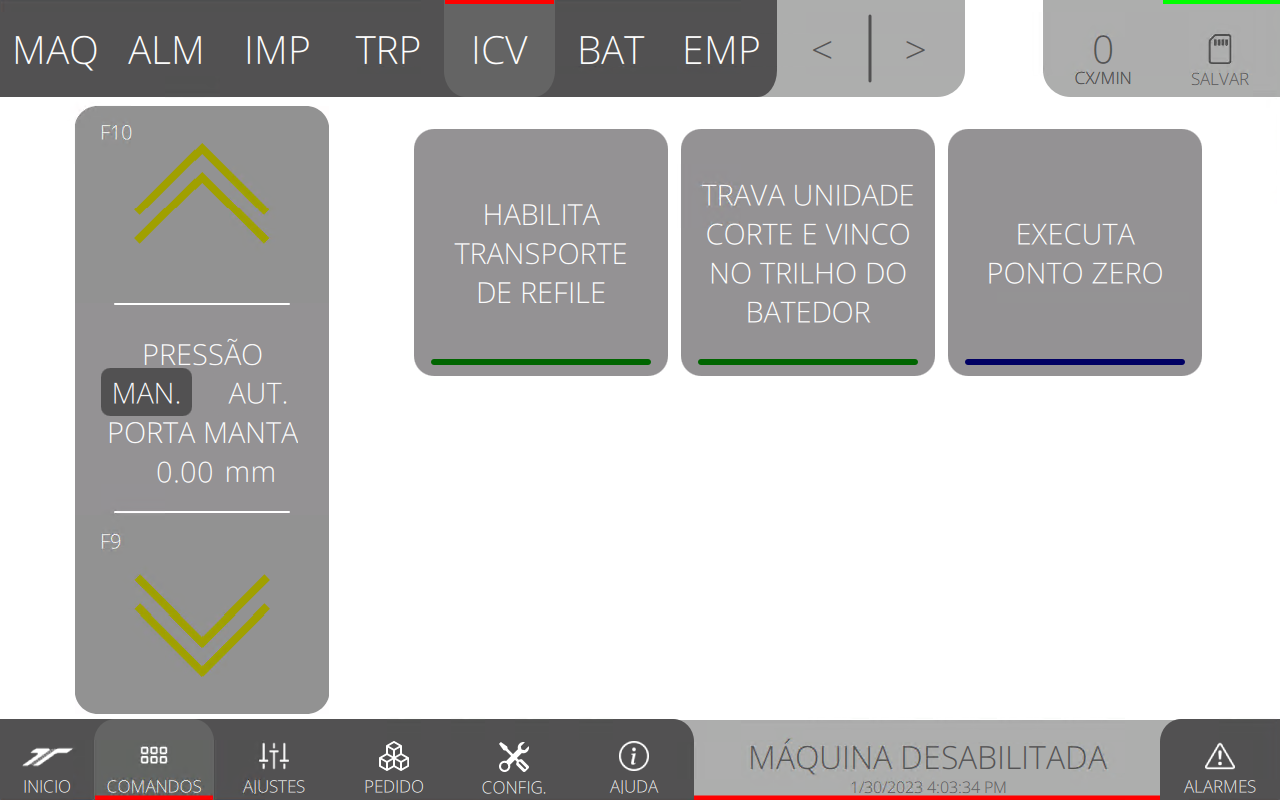
\includegraphics[width=480 px,height=300 px]{src/imagesICV/06-dryCutter/commands/e-Tela-Principal.png}
\end{figure}
\vspace*{\fill}

\newpage
\thispagestyle{fancy}
\vspace*{40 pt}
\subsubsection{\small{Ajuste de pressão no Porta Manta}} \label{sec:comandosCorteVincoAjustePressaoPortaManta}
\vspace*{\fill}
\begin{figure}[h]
    \centering
    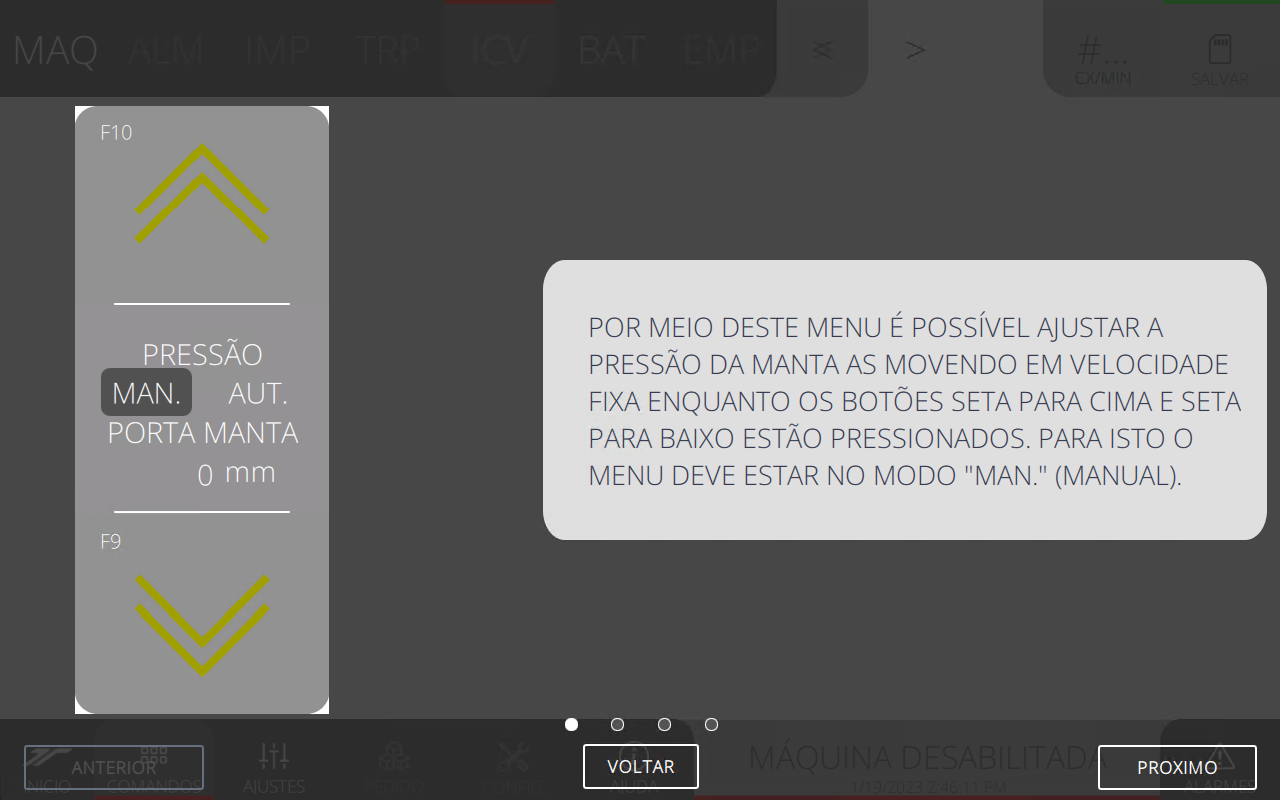
\includegraphics[width=576 px,height=360 px]{src/imagesICV/06-dryCutter/commands/e-1.png}
\end{figure}
\vspace*{\fill}

\newpage
\thispagestyle{fancy}
\vspace*{40 pt}
\subsubsection{\small{Executa ponto zero}} \label{sec:comandosCorteVincoExecutaPontoZero}
\vspace*{\fill}
\begin{figure}[h]
    \centering
    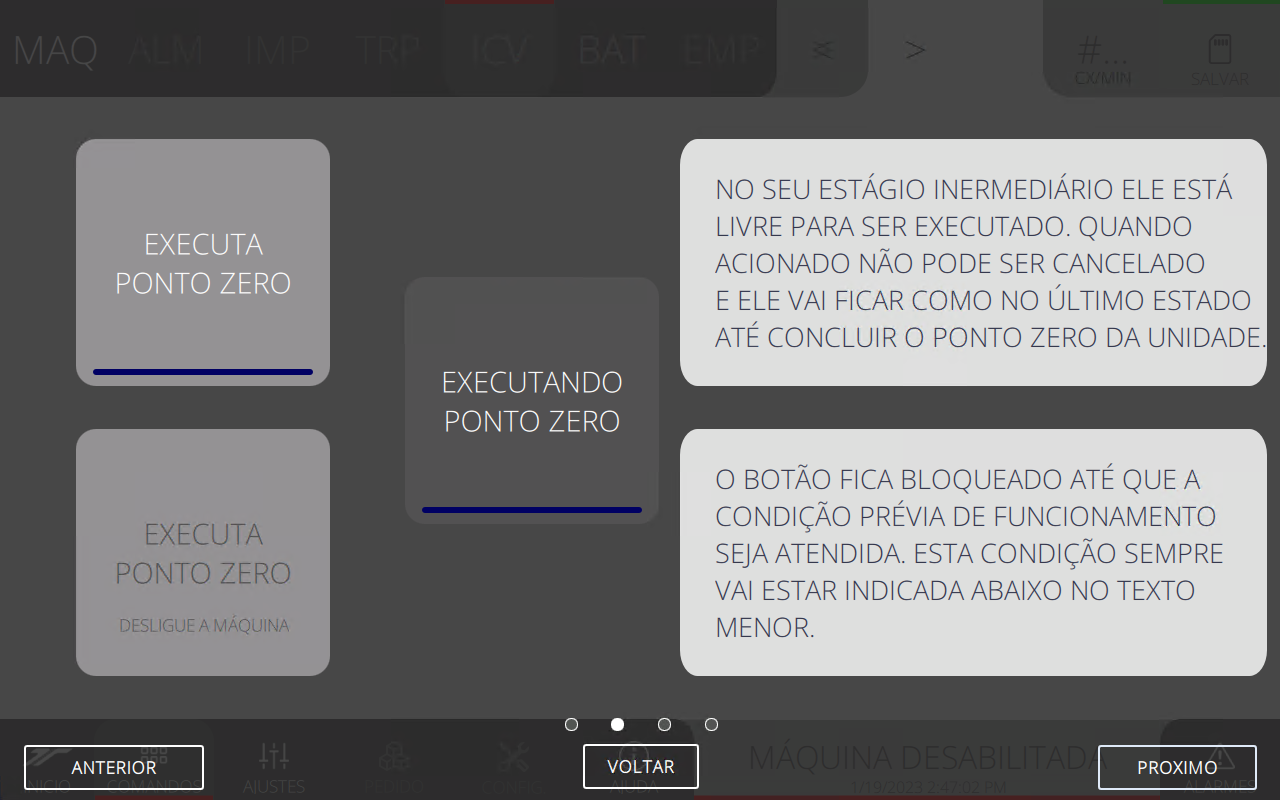
\includegraphics[width=576 px,height=360 px]{src/imagesICV/06-dryCutter/commands/e-2.png}
\end{figure}
\vspace*{\fill}

\newpage
\thispagestyle{fancy}
\vspace*{40 pt}
\subsubsection{\small{Trava unidade Corte e Vinco na unidade Batedor}} \label{sec:comandosCorteVincoTravaUnidadeCorteVincoUnidadeBatedor}
\vspace*{\fill}
\begin{figure}[h]
    \centering
    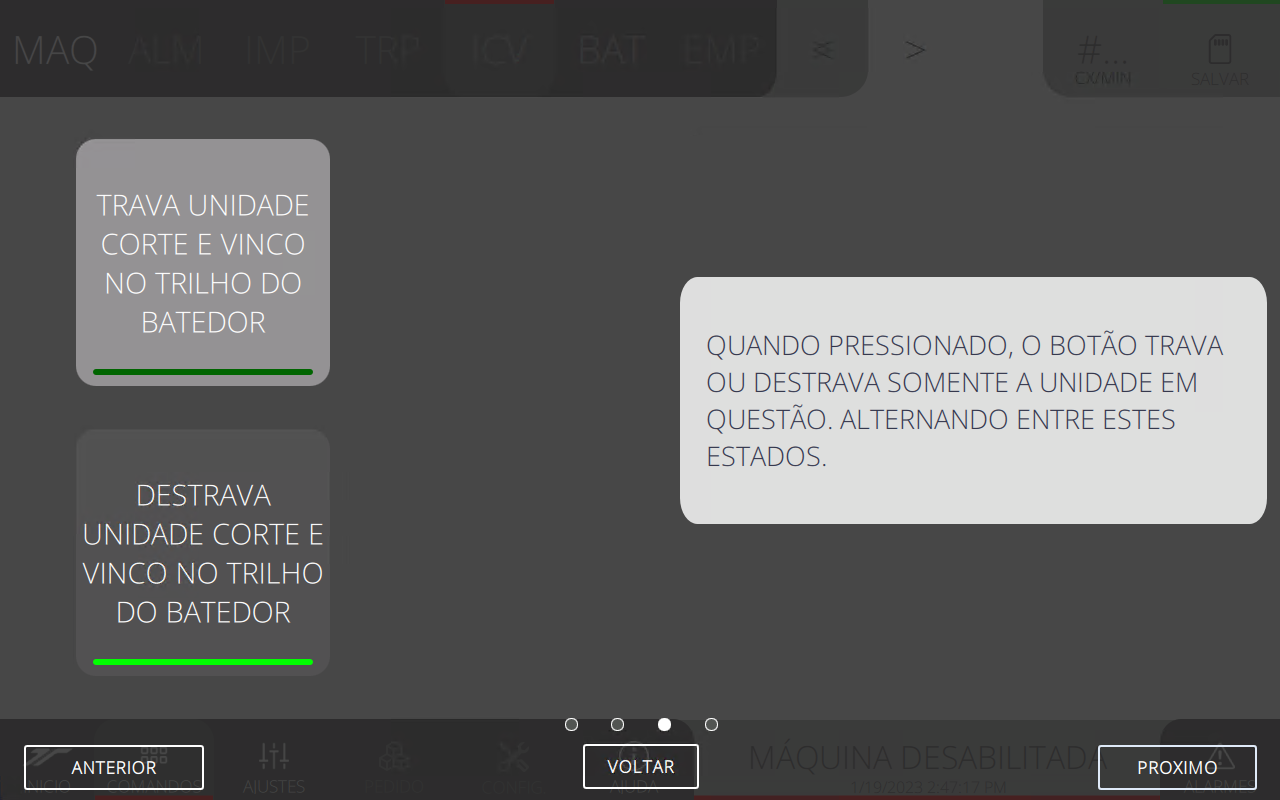
\includegraphics[width=576 px,height=360 px]{src/imagesICV/06-dryCutter/commands/e-3.png}
\end{figure}
\vspace*{\fill}

\newpage
\thispagestyle{fancy}
\vspace*{40 pt}
\subsubsection{\small{Habilita transporte de refiles}} \label{sec:comandosCorteVincoHabilitaTransporteRefiles}
\vspace*{\fill}
\begin{figure}[h]
    \centering
    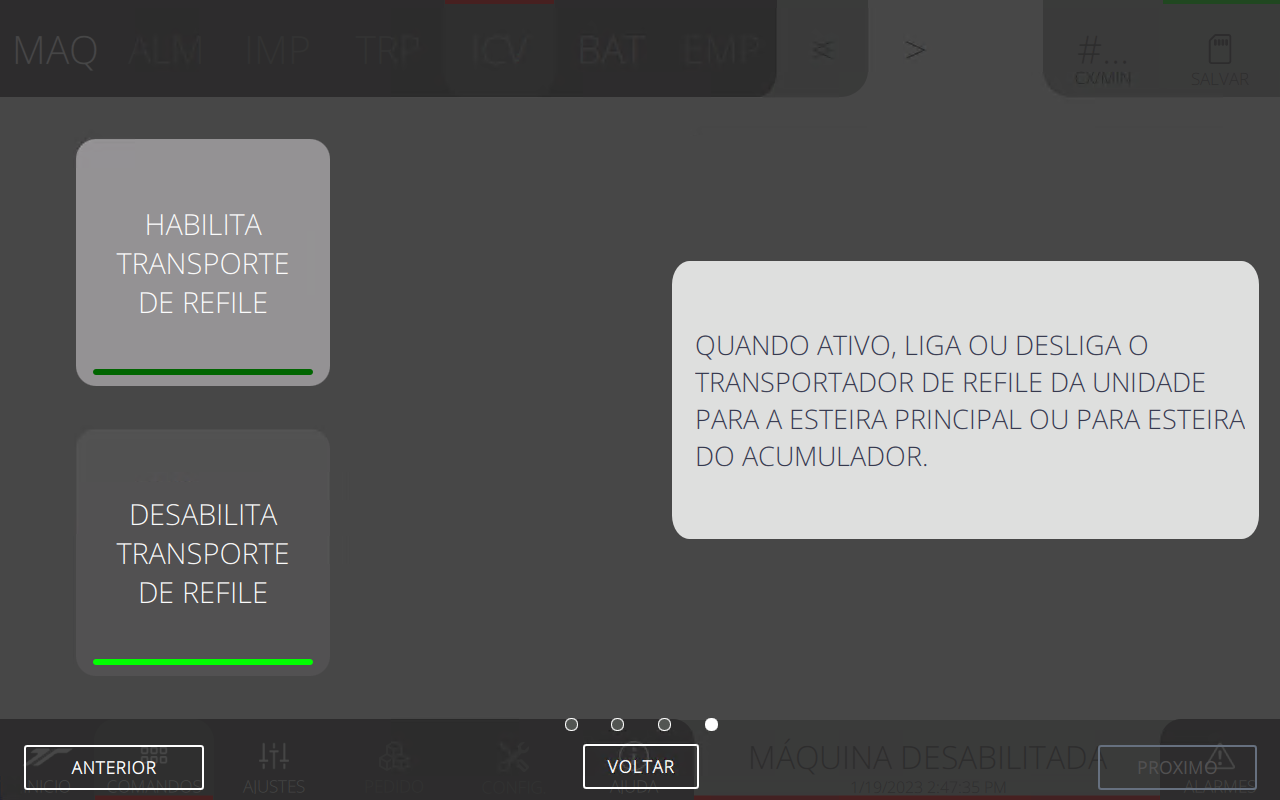
\includegraphics[width=576 px,height=360 px]{src/imagesICV/06-dryCutter/commands/e-4.png}
\end{figure}
\vspace*{\fill}